\section{Magnetfeldabhängigkeit}
\subsection{Messwerte}
Um die Magnetfeldabhängigkeit der des maximalen Josephson-Stromes \(I_C\) zu bestimmen, wurden unterschiedliche Spannungen am Helmholtz-Spulenpaar angelegt und die Strom-Spannungs-Kennlinien aufgenommen. Eine representative Kennlinie ist in \cref{fig:b-dependence} dargestellt.
Dabei wurden die Magnetfeldstärken über \cref{eq:Spule} mit dem Verhältnis \(n/R=2144\text{Wdg/m}\) berechnet.

\begin{figure}
    \centering
    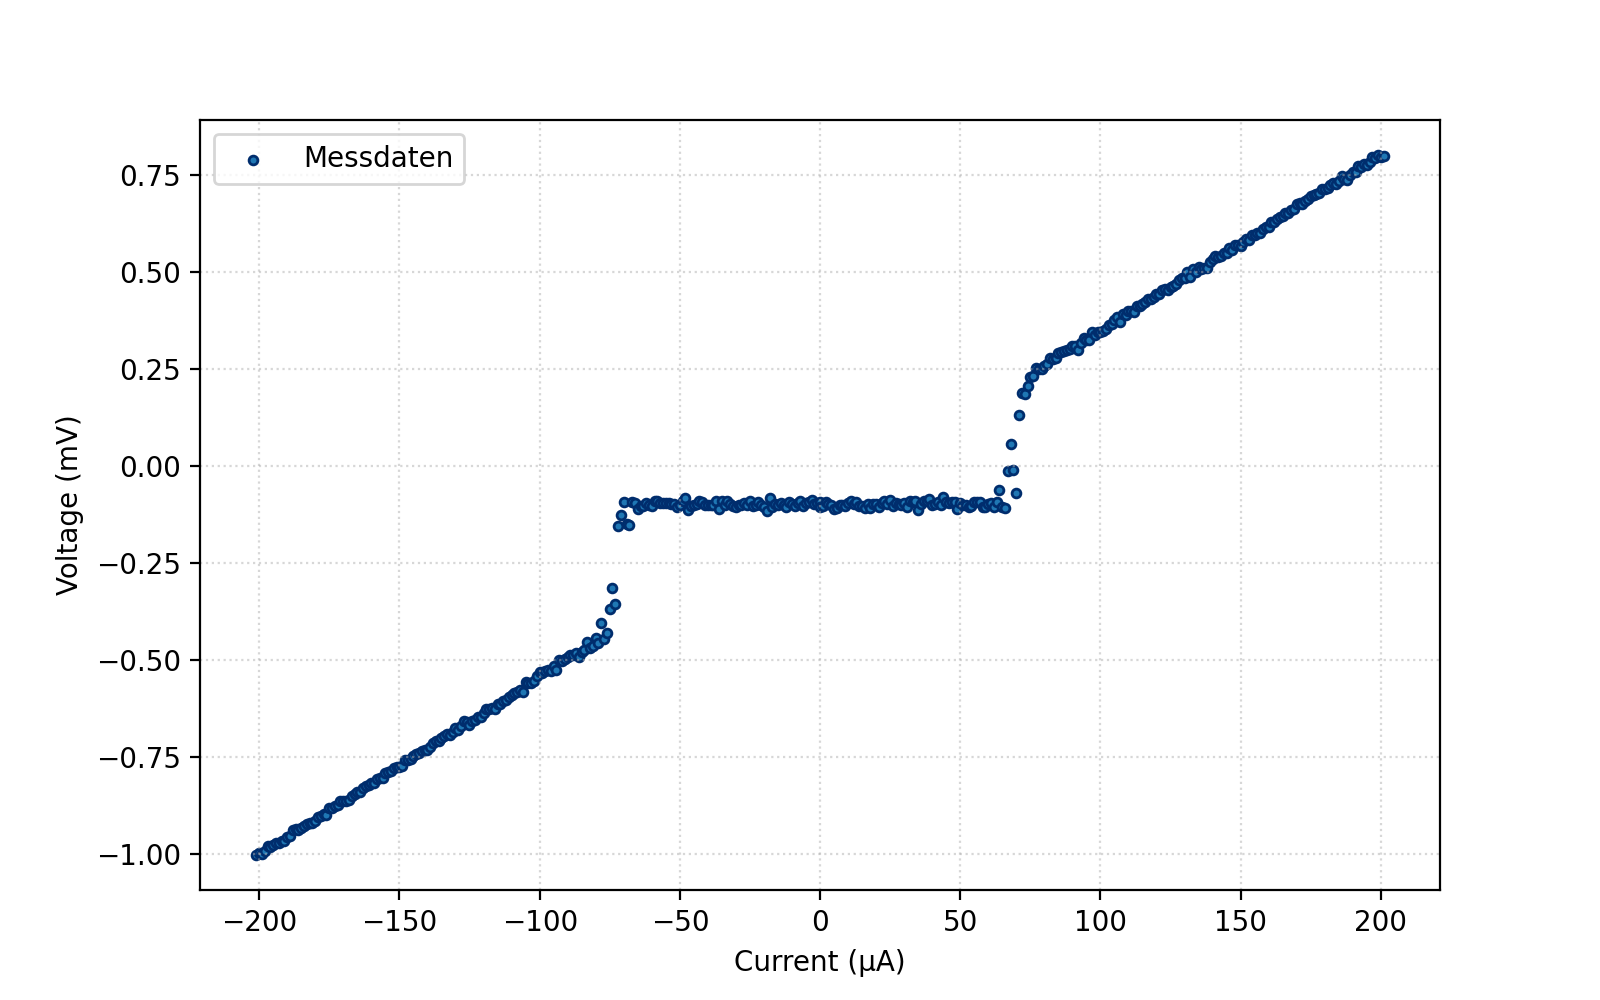
\includegraphics[width=.8 \linewidth]{measurements/eval_B/simple_curve.png}
    \caption{Aufgenommene Spannung-Strom-Kennlinie für eine angelegte Spulenspannung von \SI{-0.5}{\volt} bei \SI{4.2}{\kelvin}. Die Sprünge bei \(V = \pm 2\Delta/e\) sind deutlich zu erkennen.}
    \label{fig:b-dependence}
\end{figure}

\begin{figure}
    \centering
    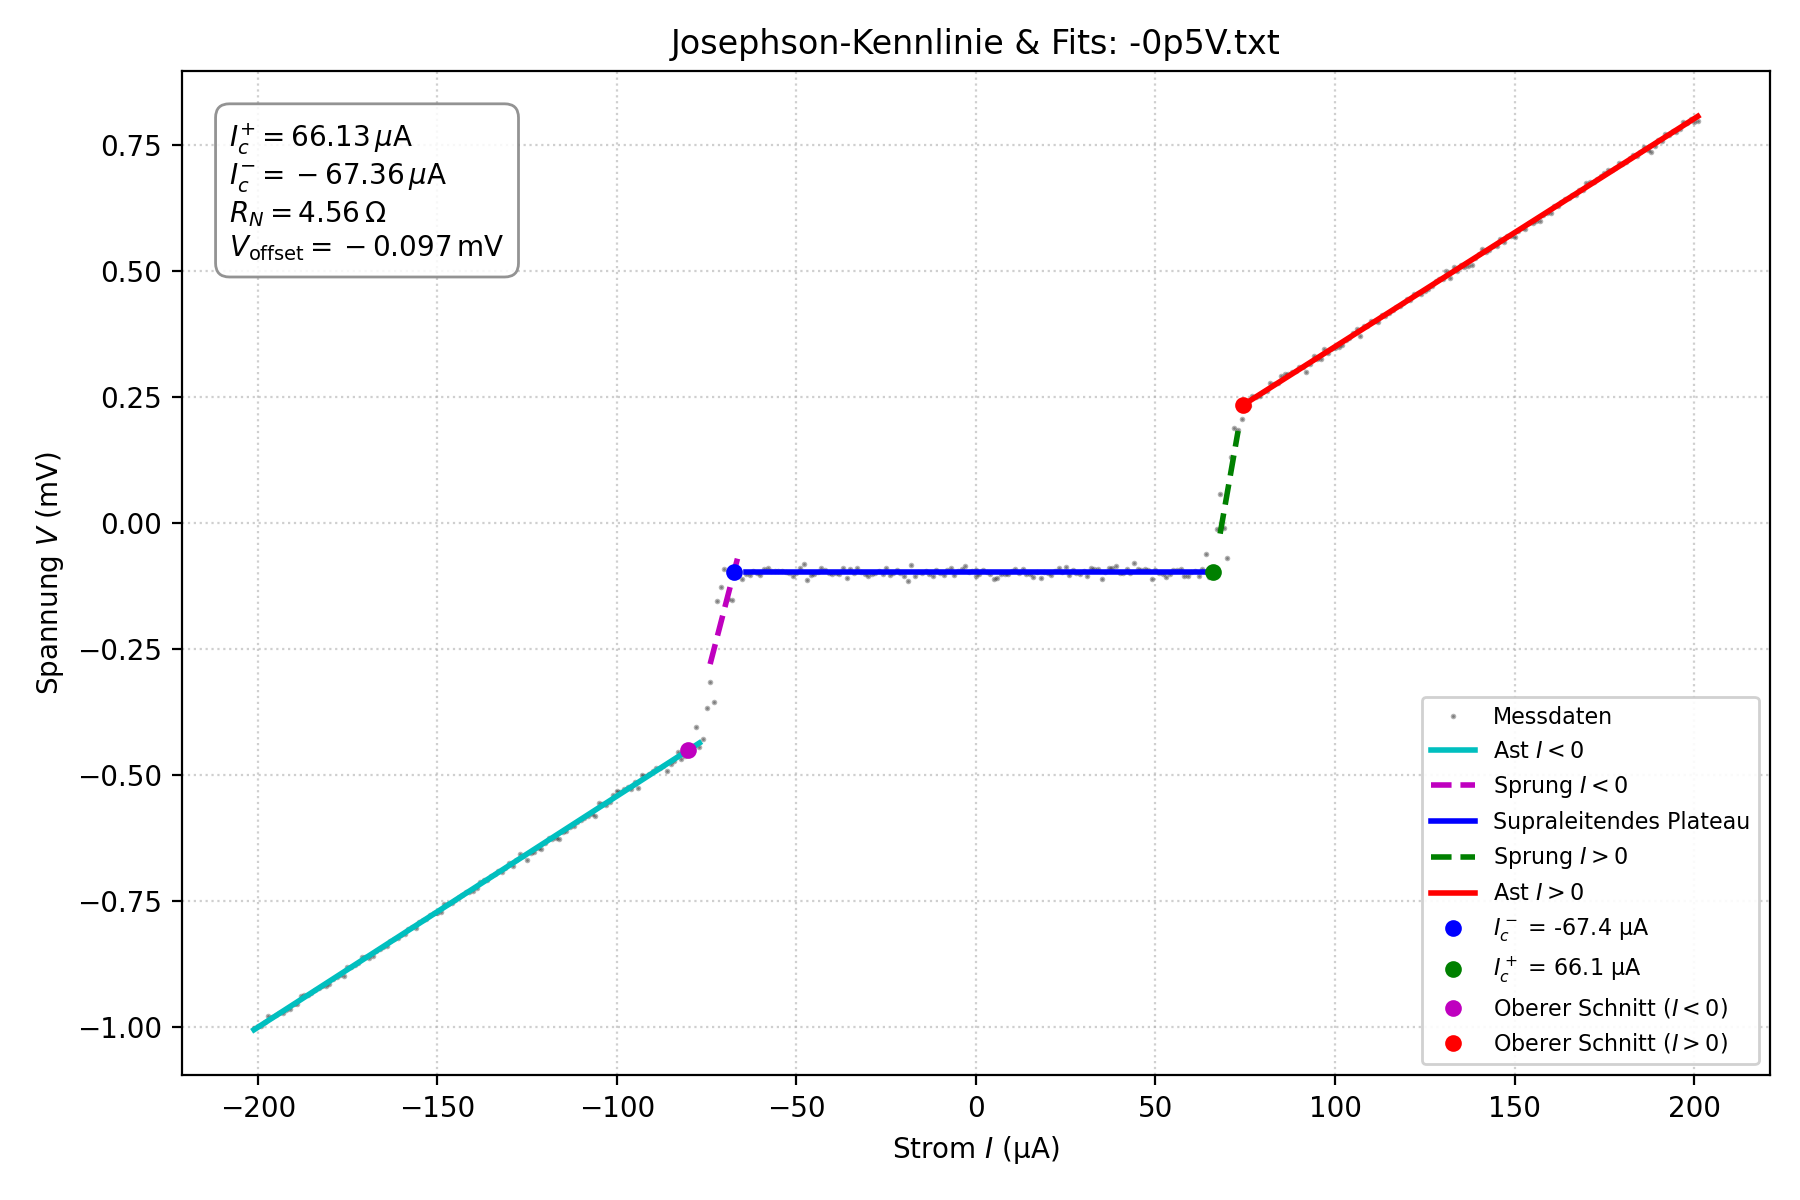
\includegraphics[width=.8 \linewidth]{measurements/eval_B/plots/fit_-0p5V.png}
    \caption{Aufgenommene Strom-Spannungs-Kennlinie bei einer Spulenspannung von \SI{-0.5}{\volt} und einer Temperatur von \SI{4.2}{\kelvin}. Die durchgezogenen bzw. gestrichelten Linien zeigen die linearen Ausgleichsgeraden der einzelnen Kennlinienabschnitte.}
    \label{fig:b-dependence-fit}
\end{figure}

Aus den Kennlinien wurde der jeweilige maximale Josephson-Strom bestimmt und gegen die Magnetfeldstärke aufgetragen. Ein repräsentativer Plot ist in \cref{fig:b-dependence} dargestellt. Die Auswertung der aufgenommenen Messkurven erfolgte durch numerische Bestimmung der lokalen Steigungsmaxima ($\mathrm{d}V/\mathrm{d}I$). Es wurden die Sprungbereiche bestimmt, die einzelnen Abschnitte separat linear gefittet und die kritischen Ströme $I_c^\pm$ als Schnittpunkte des supraleitenden Plateaus mit den jeweiligen Sprungflanken extrahiert (beispielhaft dargestellt in \cref{fig:b-dependence-fit}). Der Verlauf des Frauenhofer-Patterns wurde an die Ergebnisse gefittet (\cref{eq:fraunhofer}). Daraus ergaben sich die Fitparameter aus \cref{tab:josephson_fit_ergebnisse}.

Auffällig sind die vergrößerten Fehlerbalken des kritischen Stroms $I_c$ im Bereich um das Hauptmaximum ($B \approx \SI{0}{\milli\tesla}$). Dies lässt sich auf zwei Faktoren zurückführen:

Zum einen erreicht der Kontakt bei verschwindendem Magnetfeld seine maximale Josephson-Kopplungsenergie. In diesem Bereich zeigt der Übergang vom supraleitenden Plateau in den resistiven Zustand experimentell keinen ideal scharfen Spannungssprung, sondern eine endliche Flankenbreite zum Beispiel durch thermisches Rauschen. 
Zum anderen basiert die Bestimmung von $I_c$ in der Auswertung auf dem Schnittpunkt zweier linearer Fits (supraleitendes Plateau und Sprungflanke). Eine geringere Flankensteilheit sowie eine erhöhte Streuung der Messpunkte im Übergangsbereich führen über die Fehlerfortpflanzung der Fitparameter zu einer deutlich größeren Unsicherheit des berechneten Schnittpunkts auf der Stromachse. Bei höheren Magnetfeldern sinkt $I_c$, wodurch der Übergang schärfer abgegrenzt ist und die Schnittpunktbestimmung wieder mit geringeren Fehlern konvergiert.

\begin{table}[htbp]
  \centering
  \caption{Zusammenfassung der extrahierten Fit-Parameter aus der Anpassung des Fraunhofer-Musters.}
  \label{tab:josephson_fit_ergebnisse}
  \begin{tabular}{llcl}
    \toprule
    Physikalische Größe & Symbol & Wert mit Unsicherheit & Einheit \\
    \midrule
    Max. Josephson-Strom     & $I_c$               & \num{0.0591 \pm 0.0035}          & \si{mA} \\
                             &                     & \num{59.09 \pm 3.53}             & \si{\micro A} \\ \addlinespace
    Magnetisches Feld-Offset & $B_{\text{offset}}$ & \num{-0.0052 \pm 0.0137}         & \si{mT} \\ \addlinespace
    Periodizität             & $\Delta B$          & \num{1.0907 \pm 0.0191}          & \si{mT} \\ \addlinespace
    Konstanter Strom-Offset  & $C$                 & \num{0.0093 \pm 0.0010}          & \si{mA} \\
                             &                     & \num{9.29 \pm 1.05}              & \si{\micro A} \\ \addlinespace
    Effektive Fläche         & $A_{\text{eff}}$    & \num{1.8959 \pm 0.0332 e-12}     & \si{m^2} \\
                             &                     & \num{1.8959 \pm 0.0332}          & \si{\micro m^2} \\
    \bottomrule
  \end{tabular}
\end{table}

%% evtl Tabelle

\begin{figure}
    \centering
    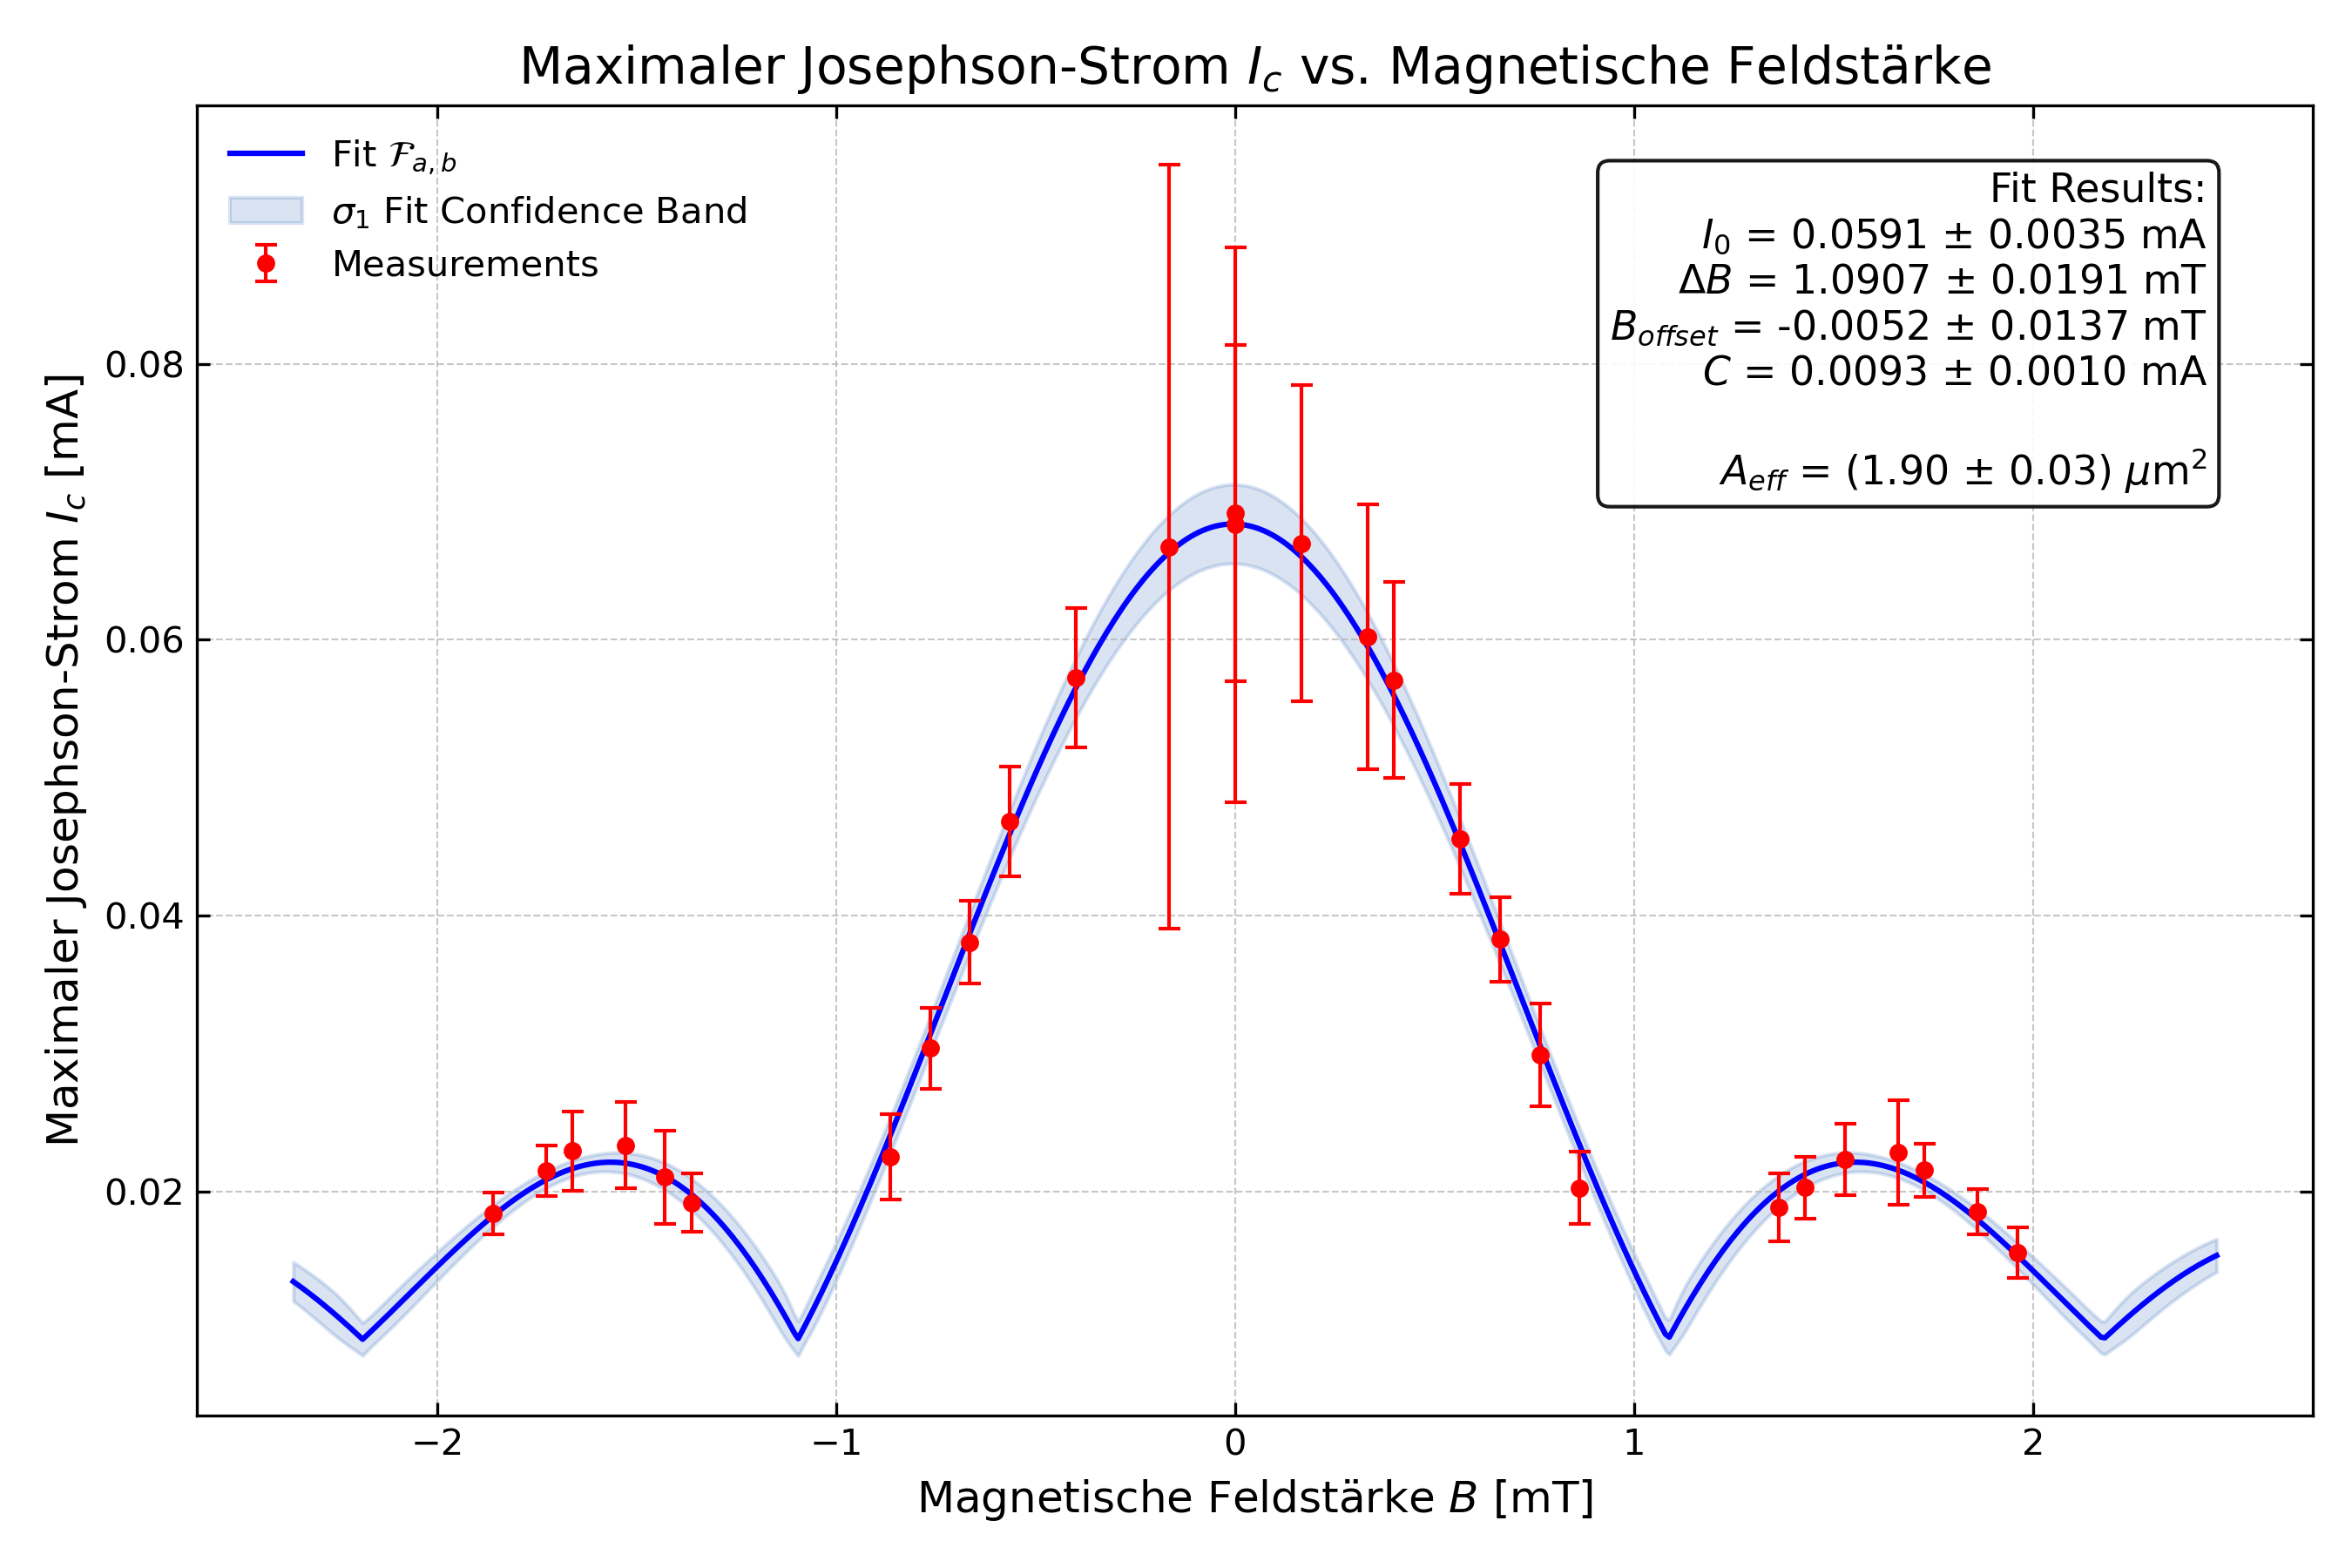
\includegraphics[width=.8 \linewidth]{measurements/eval_B/fraunhofer_fit.png}
    \caption{Maximaler Josephson-Strom \(I_C\) in Abhängigkeit der angelegten Magnetfeldstärke de Helmholtz-Spulen. Der Verlauf des Frauenhofer-Patterns wurde an die Ergebnisse gefittet. Zusätzlich sind noch die Konfidenzintervalle für \(\sigma_1\) basierend auf den Fehlern der Fits für die maximalen Josephson-Ströme dargestellt.}
    \label{fig:fraunhofer-plot}
\end{figure}

Der aus dem Fit extrahierte maximale Josephson-Strom bei verschwindendem effektiven Magnetfeld beträgt $I_c = (59.09 \pm 3.53)\ \mu\text{A}$ (bzw. $0.0591 \pm 0.0035\ \text{mA}$). Dieser Wert ist proportional zur Energielücke \(\Delta(T)\) des Supraleiters.
Für das magnetische Feld-Offset ergibt sich ein Wert von $B_{\text{offset}} = (-5.2 \pm 13.7)\ \mu\text{T}$ (bzw. $-0.0052 \pm 0.0137\ \text{mT}$). Ein solches Feld-Offset resultiert physikalisch aus dem ungeschirmten Anteil des externen Erdmagnetfeldes (typischerweise im Bereich von $30\ \mu\text{T}$ bis $60\ \mu\text{T}$).
Hierbei übersteigt die Unsicherheit den Wert des Offsets, sodass das Ergebnis mit einem Offset von null vereinbar ist.
Die Periodizität der Oszillation, welche dem Durchtritt eines magnetischen Flussquants $\Phi_0$ durch die effektive Barrierefläche entspricht, beträgt $\Delta B = (1.0907 \pm 0.0191)\ \text{mT}$.
Mit dem magnetischen Flussquant $\Phi_0 = \frac{h}{2e} \approx 2.0678 \times 10^{-15}\ \text{Vs}$ lässt sich die effektive Fläche des Josephson-Kontaktes berechnen:

\begin{equation}
    A_{\text{eff}} = \frac{\Phi_0}{\Delta B} = (1.8959 \pm 0.0332)\ \mu\text{m}^2
\end{equation}

Des weiteren gilt der Zusammenhang zur Londonschen Eindringtiefe

\begin{equation}
    A_{\text{eff}} = w \cdot (D + \lambda_{L,1} + \lambda_{L,2}) = w \cdot (D + 2 \lambda_{L})
\end{equation}
wobei \(\lambda_{L,1} = \lambda_{L,2} = \lambda_{L} \). Mit den Probenabmessungen von $w = 10\ \mu\text{m}$ und $D = 30\ \text{nm}$ ergibt sich ein Wert von

\begin{equation}
    \lambda_L = \frac{1}{2} \left( \frac{A_{\text{eff}}}{w} - D \right) = (79.79 \pm 1.66)\ \text{nm}
\end{equation}
Ein Literaturwert aus \cite{kittel} ist \(\lambda_{\text{Literatur}} = 39nm\). 
Die kritische Stromdichte $j_c$ normiert den maximalen Josephson-Strom auf die geometrische Kontaktfläche (mit $A_{\text{geo}} = w \cdot L = 100\ \mu\text{m}^2$):

\begin{equation}
j_c = \frac{I_0}{w \cdot L} = (5909.30 \pm 352.51)\ \text{A/cm}^2
\end{equation}

Aus $j_c$ und der magnetischen Dicke $d_{\text{mag}} = D + 2\lambda_L$ lässt sich die Josephson-Eindringtiefe $\lambda_J$ berechnen.

\begin{equation}
\lambda_J = \sqrt{\frac{\Phi_0}{2\pi \mu_0 d_{\text{mag}} j_c}} = (48.35 \pm 1.50)\ \mu\text{m}
\end{equation}

Da das Verhältnis der Kontaktlänge $L$ zur Josephson-Eindringtiefe $\lambda_J$

\begin{equation}
\frac{L}{\lambda_J} = 0.2068 \pm 0.0064 \ll 1
\end{equation}

befindet sich der untersuchte Josephson-Kontakt im Short-Junction-Limit (kurzer Kontakt).
Da die geometrische Ausdehnung $L = 10\ \mu\text{m}$ deutlich kleiner als die charakteristische Abschirmungslänge $\lambda_J \approx 48\ \mu\text{m}$ ist, kann der fließende Josephson-Strom das im Kontakt herrschende Magnetfeld nicht nennenswert abschirmen.
Der räumliche Verlauf der supraleitenden Phase $\varphi(x)$ entlang des Kontakts ist in  Näherung linear und wird ausschließlich durch das homogene externe Magnetfeld bestimmt.
Diese Linearität ist die mathematische Voraussetzung für die mathematische Fourier-Transformation, die zur idealen Fraunhofer-Form ($I_c \propto \vert{}\text{sinc}(x)\vert{}$) führt. Wäre $L \ge \lambda_J$, würde das Interferenzmuster stark verzerren. Die Anpassbarkeit unserer Daten bestätigt das Vorliegen des Short-Junction-Limits experimentell.